\chapter{Shaft Design}
\section{Nomenclature}
\begin{tabular}[t]{lp{7cm}}
	$ [\tau] $ & permissible torsion, $ \unit{MPa} $\\
	$ r $ & position of applied force on the shaft, $\unit{mm}$\\
	$ hr $ & tooth direction\\
	$ cb $ & role of gear on the shaft (active or passive)\\
	$ cq $ & rotational direction of the shaft\\
	$ \sigma_b $ & ultimate strength, $ \unit{MPa} $\\
	$ \sigma_{ch} $ & yield limit, $ \unit{MPa} $\\
	$ S $ & safety factor\\
	$ F_x $ & applied force, $ \unit{N} $\\
	$ F_t $ & tangential force, $ \unit{N} $\\
	$ F_r $ & radial force, $ \unit{N} $\\
	$ F_a $ & axial force, $ \unit{N} $\\
	$ a_w $ & shaft distance, $ \unit{mm} $\\
	$ d $ & shaft diameter, $ \unit{mm} $\\
	$ d_w $ & gear diameter, $ \unit{mm} $\\
	
\end{tabular}
\begin{tabular}[t]{lp{7cm}}
	$ q $ & standardized coefficient of shaft diameter\\
	$ b_O $ & rolling bearing width, $ \unit{mm} $\\
	$ l_m $ & hub diameter, $ \unit{mm} $\\
	$ T $ & torque on shaft\\
	$ \alpha_{tw} $ & meshing profile angle, $ ^\circ $\\
	$ \beta $ & helix angle, $ ^\circ $\\
	$ _1 $ & subscript for shaft 1\\
	$ _2 $ & subscript for shaft 2\\
	$ _x $ & subscript for x-axis\\
	$ _y $ & subscript for y-axis\\
	$ _z $ & subscript for z-axis\\
	$ _{sh1} $ & subscript for shaft 1\\
	$ _{sh2} $ & subscript for shaft 2\\
\end{tabular}
\section{Choose material}
For moderate load, we will use quenched steel 40X to design the shafts. From table 6.1, the specifications are as follows: $ S \leq 100\unit{(mm)} $, HB260, $ \sigma_b = 850\unit{(MPa)}$, $ \sigma_{ch} = 550\unit{(MPa)}$. 

\section{Tranmission Design}
\subsection{Load on shafts}
\subsubsection{Applied forces from Gears}
Following p.186, the subscript convention of the book will be used in this chapter. If a symbol has 2 numeric subscripts, the first one is the ordinal number of shafts while the second one is used for machine elements. On shaft 1, the motor is labeled 1 and the pinion is labeled 2. On shaft 2, the driven gear is labeled 1 and the driving sprocket is labeled 2. Therefore, we obtain:\\
$ r_{12} = d_{w12}/2 \approx 13.57\unit{(mm)}$, $ hr_{12} = +1 $, $ cb_{12} = +1 $, $ cq_1 = +1 $\\
$ r_{21} = d_{w21}/2 \approx 67.84\unit{(mm)}$, $ hr_{21} = +1 $, $ cb_{21} = -1$, $ cq_2 = -1$
\paragraph{Find magnitude of $ F_{t} $, $ F_r $, $ F_a $}
Using the results from the previous chapter: $ \alpha_{tw} \approx 21.17^\circ $, $ \beta = 20^\circ $, $ d_{w12}\approx 27.14\unit{(mm)} $
\[
\left\{ 
\begin{array}{l@{{}={}}l@{{}={}}l}
F_{t12}& F_{t21}& \dfrac{2T_{sh1}}{d_{w12}}\approx 2769.03\unit{(N)}\\
F_{r12}& F_{r21}&  \dfrac{F_{t12}\tan\alpha_{tw}}{\cos\beta}\approx1141.36\unit{(N)}\\
F_{a12}& F_{a21}& F_{t12}\tan\beta\approx1007.84\unit{(N)}\\ 
\end{array}
\right.
\]
\paragraph{Find direction of $ F_{t} $, $ F_r $, $ F_a $}
Following the sign convention, we obtain the forces:
\[
\left\{ 
\begin{array}{l@{{}={}}l}
F_{x12}& \dfrac{r_{12}}{|r_{12}|}cq_1cb_{12}F_{t12}\approx2769.03\unit{(N)}\\

F_{y12}& -\dfrac{r_{12}}{|r_{12}|}\dfrac{\tan\alpha_{tw}}{\cos\beta}F_{t12}\approx-1141.36\unit{(N)}\\

F_{z12}& cq_1cb_{12}hr_{12}F_{t12}\tan\beta\approx1007.84\unit{(N)}\\ 
\end{array}
\right.
\]
\[
\left\{ 
\begin{array}{l@{{}={}}l}
F_{x21}& \dfrac{r_{21}}{|r_{21}|}cq_2cb_{21}F_{t21}\approx2769.03\unit{(N)}\\

F_{y21}& -\dfrac{r_{21}}{|r_{21}|}\dfrac{\tan\alpha_{tw}}{\cos\beta}F_{t21}\approx-1141.36\unit{(N)}\\

F_{z21}& cq_2cb_{21}hr_{21}F_{t21}\tan\beta\approx1007.84\unit{(N)}\\ 
\end{array}
\right.
\]

\subsubsection{Applied forces from Chain drives}
Assuming the angle between x-axis and $ F_r $ is $ 150^\circ $ and $ F_r \approx 2539.28\unit{(N)} $ (chapter 2), we get the direction of $ F_r $ on shaft 2:
\[
\left\{ 
\begin{array}{l@{{}={}}l}
F_{x22}& F_{r22}\cos150^\circ\approx-2199.08\unit{(N)}\\

F_{y22}& F_{r22}\sin150^\circ\approx1269.64\unit{(N)}\\
\end{array}
\right.
\]

\subsection{Preliminary calculations}
Since shaft 1 receives input torque $ T_{sh1} $ and shaft 2 is produces output torque $ T_{sh2} $, $ [\tau_1] = 15\unit{(MPa)}$ and $ [\tau_2]=30\unit{(MPa)} $. Using equation (10.9), we can approximate $ d_1 $ and $ d_2 $:\\
$ d_1 \geq \sqrt[3]{\dfrac{T_{sh1}}{0.2[\tau_1]}} \approx 23.22\unit{(mm)}\Rightarrow d_1 = 25\unit{(mm)}$\\
$ d_2 \geq \sqrt[3]{\dfrac{T_{sh2}}{0.2[\tau_2]}} \approx 30.99\unit{(mm)}\Rightarrow d_1 = 35\unit{(mm)}$
\subsection{Identify the distance between bearings and applied forces}
From table (10.2), we can estimate $ b_O $. On shaft 1, $ b_{O1} = 15\unit{(mm)} $. On shaft 2, $ b_{O2} = 21\unit{(mm)} $. Using equation (10.10), $ l_{m1} = 1.5d_1 \approx  34.83\unit{(mm)} $, $ l_{m2} = 1.5d_2 \approx 46.48\unit{(mm)} $.
\begin{figure}[ht]
	\centering
	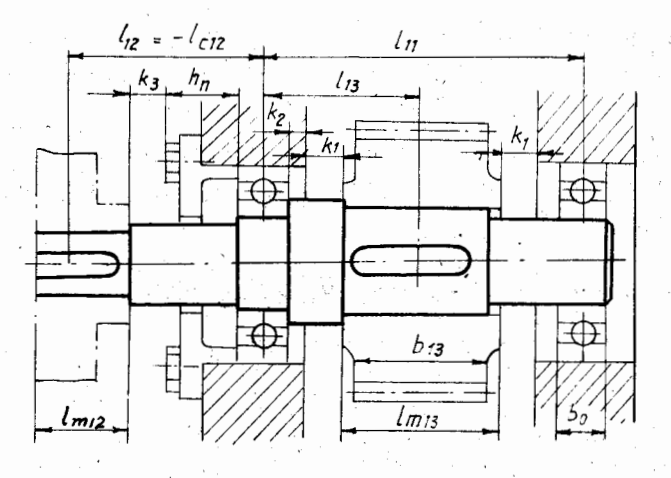
\includegraphics[width=120mm]{shaft1.png}
	\caption{Shaft design and its dimensions}
\end{figure}
%\paragraph{Find $ a_w $} On p.149, the following formula is used:
%\begin{equation}
%	a_w = (z_2+q)\sqrt[3]{\left( \dfrac{170}{z_2[\sigma_H]}\right) ^2 \dfrac{T_2K_H}{q}}
%\end{equation}